This chapter introduces this research proposal. It starts with the problem statement, then outlines the motivations, research goals and the organization of this proposal.

\section{Problem Statement}
\label{sec:statement}

\bx{Cloud computing has made a huge impact on the modern software industry by offering on-demand computing capacity 
(e.g storage and computing) \cite{2010arxiv1006.0308b}.} Compared with the traditional software industry, where applications run
on individual hardware, on-demand cloud computing provides a cluster of servers for the software industry. For example, 
web service providers, such as Google and Neflix, deploy their applications on clouds. These web service providers 
do not need to purchase and maintain hardware resources. They rent hardwares from clouds.
In addition, web service providers do not need to worry 
about scalability and availability issues when demands of their applications increase. Cloud dynamically increases the capacity of applications and cloud computing services can be accessible 99.99\% of the time~\cite{adhikari:2012uq}.
\qy{Moreover, application users} can enjoy applications without experiencing breakdown and access the applications from anywhere in the world.

\bx{A major issue in cloud computing is the huge energy consumption generated by data centers.}
A typical data center consumes as much energy as 25,000 households \cite{dayarathna:2016ua}. 
This huge energy consumption has become the major expense of cloud providers. It is necessary to find ways to reduce the energy bills. 
The reduction of energy bills would benefit \qy{cloud providers, web service providers and environment.} 
Furthermore, people would pay less to use the applications on clouds. 

\bx{Generally, cloud providers can reduce the energy consumption in clouds by
improving the resource utilization of live physical machines (PMs) such as servers.} 
Studies \cite{Barroso:2007jt, Shen:2015hm} show that \qy{PMs account for} more than 40\% of energy consumption \qy{in clouds among other components such as cooling systems and network devices}. However, studies show that PMs are not used efficiently -- the average utilization of PMs is ranging from 10\% to 50\% \cite{Hameed:2016cmb}.
Therefore, we can reduce energy by improving the average utilization of PMs \qy{and turning off the ideal PMs in clouds}.

\bx{The common way to improve the utilization of PMs in clouds 
is through resource management of PMs \cite{Manvi:2014hm} (see Figure \ref{fig:workflow}).} 
\qy{ A centralized resource management system in clouds}
has two \qy{main} functionalities. \qy{First, the management} system 
allocates resources, such as CPUs and memories of PMs, \qy{for} cloud users \qy{to run} applications. \qy{Second, the management} system 
handles the fluctuation of workloads \qy{to reduce the number of potential migrations}. \qy{These two main functionalities that directly determine the utilization of PMs in clouds.} 

\bx{The two main functionalities of resource management of PMs in clouds involve four steps.}
First, the resource management system collects and analyzes the utilization information of PMs and the resources needed by applications. Next, triggered by resource analysis, the management system determines the 
placement of applications. The placement of applications includes three scenarios: initial placement of new applications; periodic placement of existing applications; 
and dynamic placement of applications for adjusting applications in a fast manner when emergency such as overloading happen. Finally, 
the management system executes the placement decision of applications to PMs. Hence, better management of resources 
in clouds contributes towards a fewer number of PMs and thus a reduction of energy consumption.



\begin{figure}
	\centering
	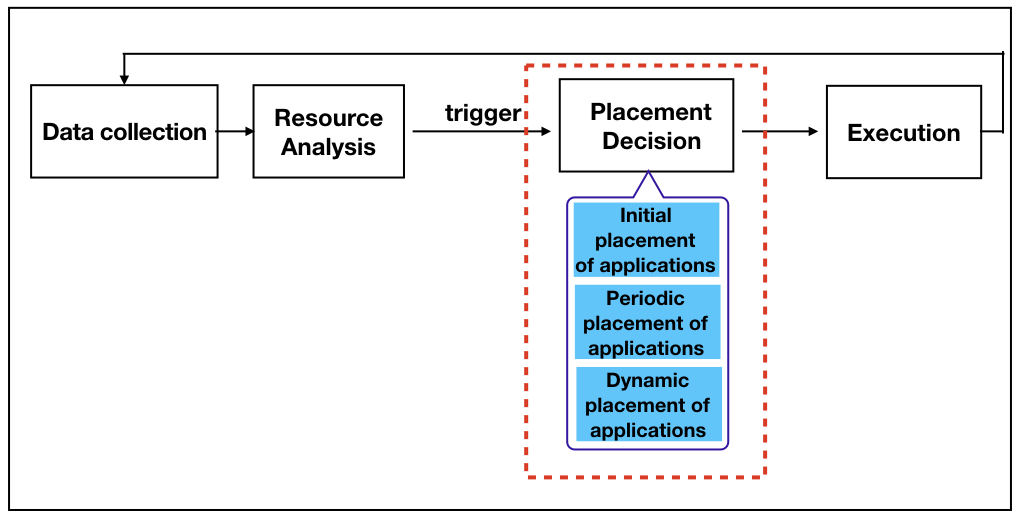
\includegraphics[width=0.8\textwidth]{pics/workflow_management.png}
	\caption{A workflow of resource management \cite{Mishra:2012kx}}
	\label{fig:workflow}
\end{figure}



\bx{The core strategy of resource management is server consolidation \cite{Varasteh:2015fu}.} Two different types of
server consolidation are used in clouds: static and dynamic. Static server consolidation manages resources in an off-line fashion. It is mainly 
used in the initial placement of applications and periodic placement of applications. Dynamic server consolidation manages resources in 
an on-line fashion. It is used in the dynamic placement of applications. Both static and dynamic server consolidation aim to place
applications in fewer PMs. This leads to fewer number of PMs with higher utilization and lower energy consumption.



\bx{Currently, server consolidation in clouds is based on \emph{virtualization} technology\cite{Uhlig:2005do} and the mainstream is virtual machine (VM)-based virtualization.}
Such virtualization separates the resources (e.g. CPUs and RAMs) of a PM into several parts called VMs. Hence, a PM can run multiple VMs and each VM runs an isolated operating system for applications. 
% This VM-based technology is very different from 
% traditional clouds that place each application to a single PM and lead to the low reserved utilization of PMs. 
% Compared with traditional clouds, current 
Therefore, VM-based clouds significantly improve the utilization of PMs and reduce the number of running PMs.


\bx{However, in recent years, VM-based virtualization cannot catch up with a new trend in the software industry -- Service Oriented Architecture 
(SOA) \cite{Sprott:2004wt}.} This SOA is widely used in the modern software industry because of its agility and re-usability \cite{Sprott:2004wt}.
SOA separates a centralized application into multiple distributed components called web services. 
As most web services only require a small amount of resources (e.g. 15\% of a typical CPU), 
using a VM for a web service causes resource wastage inside a VM. Consequently, the low utilization of PMs decreases
the energy efficiency in clouds.


\bx{To support SOA and further reduce energy consumption, a new container-based virtualization~\cite{Felter:2015ki, Soltesz:2007cu} has been proposed.} Containers running on top of 
VMs are called an operating system (OS) level of virtualization~\cite{Soltesz:2007cu}. Similar to VMs, 
containers provide performance and resource isolation for applications. 
Different to VMs, multiple containers can run in the same VM without interfering with each other. 
In addition, containers naturally support \emph{vertical scaling} (change capacity during runtime)~\cite{Vaquero:2011gb}. 
The vertical scaling provides resilient resources to the fluctuation of workloads. The container technology provides a new architecture for allocating applications and a finer granularity of resource management. Hence, containers have the potential to further
improve the utilization of PMs that leads to a high energy efficiency.



\bx{Although the use of containers provides the opportunity of improving the utilization of VMs and PMs, 
containers bring new challenges and difficulties to server consolidation~\cite{:2017ff}.} First, we cannot directly apply current VM-based server consolidation approaches to container-based server consolidation. It is because the VM-based consolidation is a one-level allocation problem: VMs-PMs while the container-based consolidation is a bilevel allocation problem: containers-VMs and VMs-PMs. These two levels of allocation interact with each other. Second, with the increasing capacity of containers, the vertical scaling in clouds requires the VMs to reserve sufficient resources. The interaction between VMs and containers changes 
the server consolidation into a bilevel allocation problem: VMs-PMs, and VMs-containers. Bilevel allocation problems are NP-hard~\cite{Sinha:2013tn} and therefore it is impossible to find the optimal solution within a reasonable amount of time. Hence, we need to use heuristics to find near optimal solutions for the bilevel allocation problem.

The aim of this research is to improve the energy efficiency in container-based clouds by proposing new bilevel energy models and server consolidation algorithms for three placement decision scenarios: 
initial placement of applications, periodic placement of applications, and dynamic placement of applications.


\vspace{5mm}
